\section{Struktur Arduino}
Perintah navigasi direktori

\section{Digital Analog}
Perintah navigasi direktori

\section{IDE}
Perintah navigasi direktori

\section{Membuat Rancangan Rangkaian}
    Membuat rangkaian dapat dilakukan dengan bantuan aplikasi simulator contohnya VBB (Virtual Bread Board). 
\begin{figure}[!htbp]
  \centering
  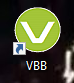
\includegraphics[width=.45\textwidth]{figures/VBB/vbb.png}
  \caption{Ini adalah aplikasi VBB}\label{fig:vbb}
\end{figure}

Bagaimana cara install VBB?
\begin{enumerate}
\item Download installer vbb
\item Double-click installer vbb,seperti pada gambar \ref{fig:installer}
\begin{figure}[!htbp]
  \centering
  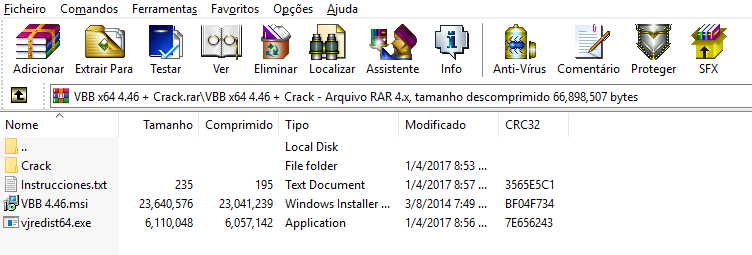
\includegraphics[width=.75\textwidth]{figures/VBB/installer.png}
  \caption{Ini adalah installer}\label{fig:installer}
\end{figure}
\item Maka akan tampil seperti gambar \ref{fig:halawalinstallasi}
\begin{figure}[!htbp]
  \centering
  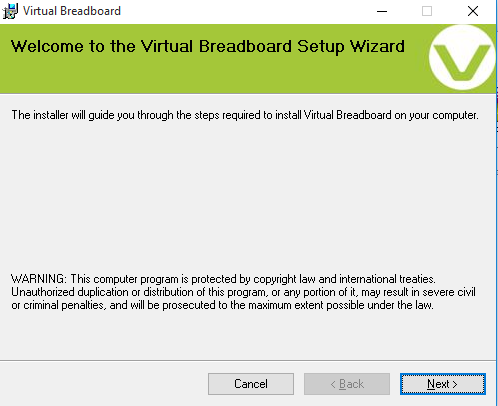
\includegraphics[width=.75\textwidth]{figures/VBB/halawalinstallasi.png}
  \caption{Ini adalah Halaman Awal Installasi}\label{fig:halawalinstallasi}
\end{figure}
\end{enumerate}